\chapter{Bisimulations of diagrams}
\label{chap:bisim}


We have seen in the previous chapter that small diagrams with values in $\R$-modules are of particular interest. Nevertheless, comparing them up to isomorphisms, i.e., morphisms $(\phi,\sigma)$ where $\phi$ is an isofunctor and $\sigma$ is a natural isomorphism, is too strong for our study of directed spaces. Indeed, the category of factorizations of the trace category contains too much information about the space. The idea would be that we want to compare homology (or homotopy) diagrams in such a way that two d-spaces have equivalent natural homology if the evolution of those diagrams with time are similar. This idea is similar to bisimulation in transition systems: systems are equivalent if they have similar evolutions of executions. We will formalize this idea using a particular instance of the fibrational views of bisimilarity evoked in section \ref{subsubsec:fibra}. We will derive several equivalent characterizations of this bisimilarity, following the different view evoked in this same section: relational definition (Section \ref{subsec:bire}) and logical definition (Section \ref{subsec:bilo}). We will also see another characterization using a extension of the Grothendieck's construction which will have no particular interest, except to relate diagrams up to bisimulations and the partially enriched categories seen in Chapter 5. Finally, in Section \ref{sec:deci}, we will look at decidability questions of this bisimilarity and of the diagramatic logic. This will use an existential theory of matrices in the reals or in the rationals both of which can be reduced to the existential theory of the reals.


\section{Fibrational bisimilarity for diagrams}

We recall first that, in the general formalism from \cite{joyal96}, one must start with a category $\M$ (of \textbf{models}) together with a subcategory $\PP$ (of \textbf{execution forms}). In our case, we will start with the category $\diagriso{\A}$ of small diagrams in a category $\A$ and whose morphisms are pairs $(\Phi,\sigma)$ where $\Phi$ is a functor and $\sigma$ is a natural isomorphism. The difference with $\diagr{\A}$ from the previous chapter is the fact that the natural transformation must be an isomorphism. For every $n \in \nat$, let $[n] = \{0, 1, \cdots,
n-1\}$, and let $i_{mn} \colon [m] \to [n]$ be the inclusion map, for $m
\leq n$.  As a poset, $[n]$ is a category, and $i_{mn}$ is then a
functor. Consider the subcategory $\PP \subseteq \diagriso{\A}$ whose objects are functors $\map F {[n]} {\A}$ and whose
morphisms from $\map H {[m]} {\A}$ to $\map F {[n]} {\A}$ are of the
form $(i_{mn}, id)$. $\diagriso{\A}$ and $\PP$ have a common initial object: the empty diagram. We can actually simplify the definition of open morphisms in this case:

	\begin{lemme}
		A morphism $\map{(\Phi,\sigma)}{(\map{F}{\C}{\A})}{(\map{G}{\D}{\A})} \in \diagriso{\A}$ is open iff it has the right lifting property with respect to $(i_{n,n+1},id)$ for all $n\in\nat$.
	\end{lemme}
	
	\begin{proof}~
		\begin{itemize}
			\item[$\Rightarrow$] by definition of open maps.
			\item[$\Leftarrow$] we show that it has the right lifting property with respect to $i_{n,m}$, using the fact that $$i_{n,m} = i_{m-1,m}\circ \ldots \circ i_{n,n+1}.$$
		\end{itemize}
	\end{proof}
	
	\begin{prop}
		A morphism $\map{(\Phi,\sigma)}{(\map{F}{\C}{\A})}{(\map{G}{\D}{\A})} \in \diagriso{\A}$ is open iff it has the right lifting property with respect to $(i_{0,1},id)$ and $(i_{1,2},id)$, i.e., iff:
		\begin{itemize}
			\item $\Phi$ is surjective on objects,
			\item for every morphism $\map{j}{d}{d'}$ of $\D$ and every $c$ of $\C$ such that $\Phi(c) = d$ there exists $\map{i}{c}{c'}$ such that $\Phi(i) = j$.
		\end{itemize}
	\end{prop}
	
	\begin{proof}~
		\begin{itemize}
			\item[$\Rightarrow$] by definition of open maps
			\item[$\Leftarrow$] Let us show that $(\Phi,\sigma)$ has the right lifting property with respect to $i_{n,n+1}$. The case $0$ is by hypothesis. Assume $n \geq 1$ and given a commutative diagram:
			\begin{center}
				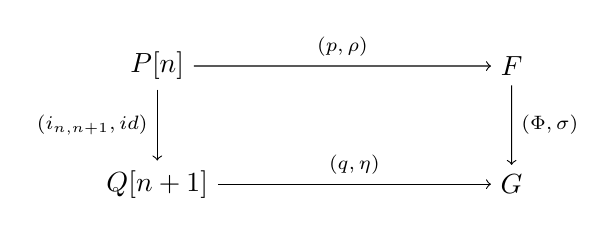
\begin{tikzpicture}[scale=1.5]
				\node (A) at (0,1) {$\map{P}{[n]}{\A}$};
				\node (B) at (3,1) {$\map{F}{\C}{\A}$};
				\node (C) at (0,0) {$\map{Q}{[n+1]}{\A}$};
				\node (D) at (3,0) {$\map{G}{\D}{\A}$};
				\path[->,font=\scriptsize]
				(A) edge node[above]{$(p,\rho)$} (B)
				(A) edge node[left]{$(i_{n,n+1},id)$} (C)
				(B) edge node[right]{$(\Phi,\sigma)$} (D)
				(C) edge node[above]{$(q,\eta)$} (D);
				\end{tikzpicture}
			\end{center}
We want $(r,\theta)$ such that: 
			\begin{center}
				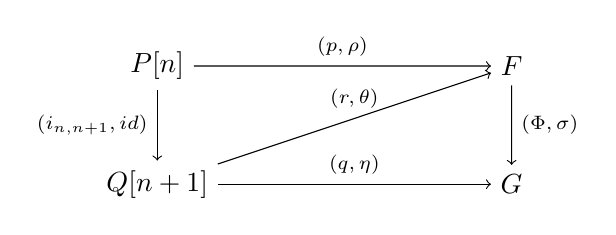
\begin{tikzpicture}[scale=1.5]
				\node (A) at (0,1) {$\map{P}{[n]}{\A}$};
				\node (B) at (3,1) {$\map{F}{\C}{\A}$};
				\node (C) at (0,0) {$\map{Q}{[n+1]}{\A}$};
				\node (D) at (3,0) {$\map{G}{\D}{\A}$};
				\path[->,font=\scriptsize]
				(A) edge node[above]{$(p,\rho)$} (B)
				(A) edge node[left]{$(i_{n,n+1},id)$} (C)
				(B) edge node[right]{$(\Phi,\sigma)$} (D)
				(C) edge node[above]{$(q,\eta)$} (D)
				(C) edge node[above]{$(r,\theta)$} (B);
				\end{tikzpicture}
			\end{center}
$\map{r}{[n+1]}{\C}$ is constructed as follow:
			\begin{itemize}
				\item for $0 \leq i \leq n-1$, $r(i) = p(i)$ and for all $j \leq i$, $r(j\leq i) = p(j \leq i)$,
				\item it remains to construct $r(n-1 \leq n)$ (which will determine $r(n)$). We know that $\map{q(n-1\leq n)}{q(n-1)}{q(n)}$ and that $q(n-1) = \Phi(p(n-1))$. Thus by the second property of $\Phi$, there exists a morphism $\map{i}{p(n-1) = r(n-1)}{c}$ of $\C$ such that $\Phi(i) = q(n-1\leq n)$. We pose $r(n-1\leq n) = i$.
			\end{itemize}
By construction $p = r \circ i_{n,n+1}$ and $\Phi\circ r = q$.\\
$\map{\theta = (\theta_i)_{0 \leq i \leq n}}{Q}{F\circ r}$ is defined as $\sigma^{-1}\circ\eta$. Consequently, it is natural isomorphism and $\sigma\circ\theta = \eta$. It remains to prove that $\theta\circ id = \rho$, i.e., for every $0 \leq i \leq n-1$, $\theta_i = \rho_i$, which is true since they are both equal to $\sigma_{q(i)}^{-1}\circ \eta_i$.
		\end{itemize}
	\end{proof}
	
	
	
Let us look at some examples. First, as we will prove later, the morphism $(\kappa_\C,\id)$ from $\nathomolbw{n}{X}$ to $\nathomolhm{n}{X}$ defined in Section \ref{sec:nathom} is always an open map, which explains why they can be used equivalently. Now, recall the first natural system of homology of $a+b$ in figure \ref{fig:bisexa} left. As we will prove later, there is a always a finite diagram that is bisimilar to $\nathomolbw{n}{X}$ when $X$ is nice enough. Such a diagram is given in figure \ref{fig:bisexa} right, and a open map from $\nathomolbw{1}{a+b}$ to this finite diagram is depicted by the color on this same figure \ref{fig:bisexa}.
		\begin{figure}[H]
			\begin{center}
    				\input{images/Bisim/Bisexa}
  			\end{center}
			\caption{Example of an open map for the first natural system of homology of $a+b$}
			\label{fig:bisexa}
		\end{figure}







\section{Relational definition}
\label{sec:reldefi}

We now turn to a more classical characterization of bisimulation for our diagrams, that relates to 
theoretical computer science and concurrency theory~: 

\begin{defi}
\label{def:alternatedefbisim}
A bisimulation $R$ between two diagrams $\map{F}{\C}{\A}$ and $\map{G}{\D}{\A}$ is a set of triples $(c,f,d)$ where $c$ is an object of $\C$, $d$ is an object of $\D$ and $\map{f}{F(c)}{G(d)}$ is an isomorphism of $\A$ such that for all $(c,f,d)$ in $R$:
\begin{itemize}
	\item if there exists $\map{i}{c}{c'} \in \C$ then there exists $\map{j}{d}{d'} \in \D$ and $\map{g}{F(c')}{G(d')} \in \A$ such that $g\circ F(i) = G(j) \circ f$ and $(c',g,d') \in R$,
	
		\begin{figure}[H]
			\begin{center}
    				
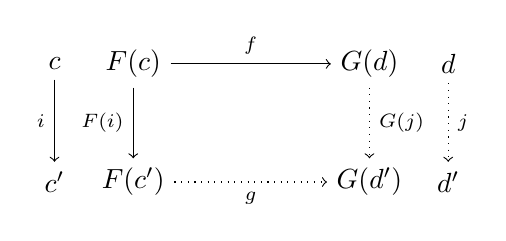
\begin{tikzpicture}[scale=1]
		
	\node (x') at (0,0) {$c'$};
   	\node (x) at (0,1.5) {$c$};
	\node (Fx') at (1,0) {$F(c')$};
	\node (Fx) at (1,1.5) {$F(c)$};
	\node (Gy') at (4,0) {$G(d')$};
	\node (Gy) at (4,1.5) {$G(d)$};
	\node (y') at (5,0) {$d'$};
   	\node (y) at (5,1.5) {$d$};
	
	\path[->,font=\scriptsize]
		(x) edge node[left]{$i$} (x')
		(Fx) edge node[left]{$F(i)$} (Fx')
		(Fx) edge node[above]{$f$} (Gy);
		
	\path[->, dotted, font = \scriptsize]
		(y) edge node[right]{$j$} (y')
		(Gy) edge node[right]{$G(j)$} (Gy')
		(Fx') edge node[below]{$g$} (Gy');
			
\end{tikzpicture}


  			\end{center}
		\end{figure}
	
	\item if there exists $\map{j}{d}{d'}\in \D$ then there exists $\map{i}{c}{c'} \in \C$ and $\map{g}{F(c')}{G(d')} \in \A$ such that $g\circ F(i) = G(j) \circ f$ and $(c',g,d') \in R$,
	
		\begin{figure}[H]
			\begin{center}
    				\input{images/Bisim/Bisim2}
  			\end{center}
		\end{figure}
	
\end{itemize}
and such that:
\begin{itemize}
	\item for all $c\in\C$, there exists $d$ and $f$ such that $(c,f,d)\in R$,
	\item for all $d\in\D$, there exists $c$ and $f$ such that $(c,f,s)\in R$.
\end{itemize}
\end{defi}

\begin{prop} Two functors $\map{F}{\C}{\M}$ and $\map{G}{\D}{\M}$ 
are bisimilar iff there exists a bisimulation between them.\end{prop}

\begin{proof}~
\begin{itemize}
	\item[$\Rightarrow$] Assume that there is a span:
	\begin{center}
	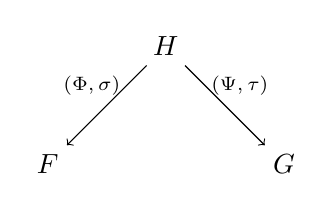
\begin{tikzpicture}[scale=1.5]
		\node (A) at (0,0) {$\map{F}{\C}{\A}$};
		\node (B) at (1,1) {$\map{H}{\E}{\A}$};
		\node (C) at (2,0) {$\map{G}{\D}{\A}$};
		\path[->,font=\scriptsize]
		(B) edge node[above]{$(\Phi,\sigma)~~~~$} (A)
		(B) edge node[above]{$~~~~(\Psi,\tau)$} (C);
	\end{tikzpicture}
	\end{center}
	of open maps. We define $R = \{(\Phi(e),\tau_e\circ\sigma^{-1}_{\Phi(e)},\Psi_e) \mid e \in \E\}$ and show that this is a bisimulation. First, it is well defined because $\tau$ and $\sigma$ are isomorphisms. The third condition of a bisimulation comes from the surjectivity of $\Phi$. Idem for the fourth and the surjectivity of $\Psi$. The first condition comes from the second condition on $\Phi$ of an open map: let $(\Phi(e),\tau_e\circ\sigma^{-1}_{\Phi(e)},\Psi_e)$ in $R$ and $\map{i}{\Phi(e)}{c'} \in \C$. By the condition on $\Phi$ there exists $\map{k}{e}{e'}$ in $\E$ such that $\Phi(k) = i$. Then define $j = \Psi(k)$, $d' = \Psi(e')$ and $g = \tau_{e'}\circ\sigma^{-1}_{\Phi(e')}$. $(\Phi(e'),g,d')$ belongs to $R$ by construction and $g\circ F(i) = G(j) \circ \tau_e\circ\sigma^{-1}_{\Phi(e)}$ by naturality of $\sigma$ and $\tau$. Idem for the second condition of a bisimulation.
	\item[$\Leftarrow$] Assume now that there is a bisimulation $R$ between $F$ and $G$. We will construct a span of open maps. Let $\E$ be the small category whose objects are elements of $R$, and
whose morphisms from $(c,f,d)$ to $(c',f',d')$ are pairs $(i,j)$
of a morphism $\map{i}{c}{c'}$ in $\C$ and of a morphism
$\map{j}{d}{d'}$ in $\D$, such that the following diagram commutes:
\begin{center}
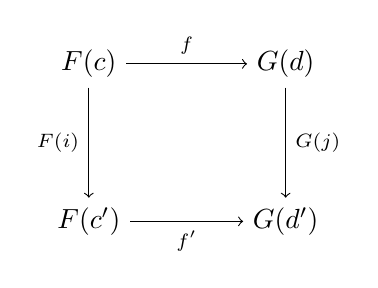
\begin{tikzpicture}
	\node (Fx') at (1,0) {$F(c')$};
	\node (Fx) at (1,2) {$F(c)$};
	\node (Gy') at (3.5,0) {$G(d')$};
	\node (Gy) at (3.5, 2) {$G(d)$};
	\path[->,font = \scriptsize]
		(Fx) edge node[left]{$F(i)$} (Fx')
		(Fx) edge node[above]{$f$} (Gy)
		(Fx') edge node[below]{$f'$} (Gy')
		(Gy) edge node[right]{$G(j)$} (Gy');
\end{tikzpicture}
\end{center}
Define the tip $H$ of the span between $F$ and $G$ as the functor
$\map{H}{E}{\A}$ that maps every object $(c,f,d)\in R$ to $F(c)$,
and every morphism $\map{(i,j)}{(c,f,d)}{(c',f',d')}$ to
$\map{F(i)}{F(c)}{F(c')}$.

We now build a morphism $(\Phi, \sigma)$ from $H$ to $F$.  We start by
building $\map{\Phi}{\E}{\C}$.  We define $\Phi$ as the functor that
maps every object $(c,f,d)$ to $c$ and every morphism
$\map{(i,j)}{(c,f,d)}{(c',f',d')}$ to $\map{i}{c}{c'}$.  We
verify that $\Phi$ satisfies the condition of the previous proposition:
\begin{enumerate}
\item $\Phi$ is surjective on objects: this is third condition of the
  definition of $R$ as a bisimulation.
\item Let $\map{i}{\Phi (e)}{c'}$ be a morphism of $X$.  The object
  $e$ must be a triple $(c,f,d) \in R$, and $i$ is a morphism from
  $c$ to $c'$ in $\C$.  By the first condition of the definition of $R$ as a
  bisimulation, there is a triple $(c',f',d') \in R$ and a morphism
  $\map{j}{d}{d'}$ of $\D$ such that the following diagram commutes:
\begin{center}
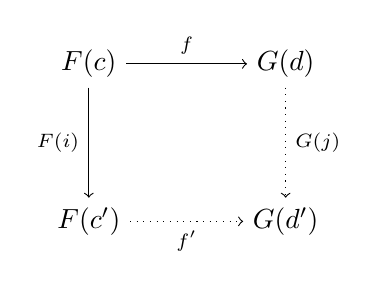
\begin{tikzpicture}
	\node (Fx') at (1,0) {$F(c')$};
	\node (Fx) at (1,2) {$F(c)$};
	\node (Gy') at (3.5,0) {$G(d')$};
	\node (Gy) at (3.5, 2) {$G(d)$};
	\path[->,font = \scriptsize]
		(Fx) edge node[left]{$F(i)$} (Fx')
		(Fx) edge node[above]{$f$} (Gy);
	\path[->, dotted, font = \scriptsize]
		(Fx') edge node[below]{$f'$} (Gy')
		(Gy) edge node[right]{$G(j)$} (Gy');
\end{tikzpicture}
\end{center}
  In particular, $(i,j)$ is a morphism of $E$, from $(c,f,d)$ to
  $(c',f',d')$.  Moreover, $H(i,j) = i$.
\end{enumerate}
For every $(c,f,d)\in R$, let $\map{\sigma_{(c,f,d)} =
  id_{F(c)}}{H(c,f,d) = F(c)}{F\circ\Phi(c,f,d) = F(c)}$.  Those
are isomorphisms, and define a natural transformation
$\map{\sigma}{H}{F\circ\Phi}$.  It follows that $(\Phi,\sigma)$ is an
open map from $H$ to $F$.\\
We define the open map $(\Psi, \tau)$ from $H$ to $G$ similarly.
\end{itemize}
\end{proof}





\section{Diagrammatic Hennessy-Milner logic}

In this section, we prove a logical characterization using a logic similar to Hennessy-Milner logic from section \ref{subsec:bilo}.

\begin{defi}[Syntax]
$$\text{\textbf{Object formulae:~~}} S::=[x]P~~~~~x\in Ob(\A)$$
$$\text{\textbf{Morphism formulae:~~}} P::=\langle f \rangle P\mid?S\mid\neg P\mid \bigwedge\limits_{i\in I} P_i~~~~~f\in Mor(\A) \text{ and } I \text{ a set}$$
\end{defi}

In the following, we will denote by $\top$ the empty conjunction, i.e., $\top = \bigwedge\limits_{i \in \varnothing} P_i$.

\begin{defi}[Semantics]
For a diagram $\map{F}{\C}{\A}$, for every object $c$ of $\C$ and for every isomorphism $f$ of $\A$ of the form $\map{f}{F(d)}{x}$ for some $d$ and $x$, we define $F,c \models S$ for an object formula $S$ and $F,f,d\models P$ for a morphism formula $P$ by induction on $S$ (resp. $P$) as follow:
\begin{itemize}
	\item $F,c \models [x]P$ iff there exists an isomorphism $\map{f}{F(c)}{x}$ of $\A$ such that $F,f,c\models P$,
	\item $F,f,c\models \langle g \rangle P$ iff $\map{g}{x}{x'}$ and there exists $\map{i}{c}{c'}$ in $\C$ and an isomorphism $\map{h}{F(c')}{x'}$ such that $h\circ F(i) = g\circ f$ and $F,h,c'\models P$,
	\begin{center}
	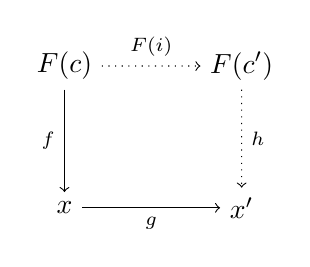
\begin{tikzpicture}[scale=1.5]
		\node (A) at (0,1.2) {$F(c)$};
		\node (B) at (1.5,1.2) {$F(c')$};
		\node (C) at (0,0) {$x$};
		\node (D) at (1.5,0) {$x'$};
		\path[->,font=\scriptsize,dotted]
		(A) edge node[above]{$F(i)$} (B)
		(B) edge node[right]{$h$} (D);
		\path[->,font=\scriptsize]
		(C) edge node[below]{$g$} (D)
		(A) edge node[left]{$f$} (C);
	\end{tikzpicture}
	\end{center}
	\item $F,f,c\models ?S$ iff $F,c\models S$,
	\item $F,f,c\models \neg P$ iff $F,f,c\not\models P$,
	\item $F,f,c\models \bigwedge\limits_{i\in I} P_i$ iff for all $i\in I$, $F,f,c\models P_i$.
\end{itemize}
We say that a diagram $\map{F}{\C}{\A}$ is \textbf{logically simulated} by another diagram $\map{G}{\D}{\A}$ if for every object $c$ of $\C$, there exists an object $d$ of $\D$ such that for all object formulae $S$, ($F,c \models S$ iff $G,d \models S$). Two diagrams $F$ and $G$ are \textbf{logically equivalent} if $F$ is logically simulated by $G$ and $G$ is logically simulated by $F$.
\end{defi}

We note that logical equivalence is an equivalence relation between diagrams.


\begin{theo}
Two diagrams are bisimilar iff they are logically equivalent.
\end{theo}

\begin{proof}~
\begin{itemize}
	\item[$\Rightarrow$] First, let us suppose that $F$ and $G$ are bisimilar. We can restrict to the case where there exists an open map $\map{(\Phi,\sigma)}{F}{G}$, the general case ensuing.
	
We prove that: 
\begin{enumerate}
	\item $(F,c\models S \Leftrightarrow G,\Phi(c)\models S)$ for all object formulae $S$ and for all objects $c$ of $\C$, 
	\item $(F,f,d\models P \Leftrightarrow G,f\circ\sigma_d^{-1},\Phi(d)\models P)$ for all morphism formulae $P$ and for all isomorphisms $\map{f}{F(d)}{x}$ of $\A$,
\end{enumerate} 
by induction on $S$ (resp. $P$).

	\begin{itemize}
		\item[$\star$] If $F,c \models [x]P$ then there exists an isomorphism $\map{f}{F(c)}{x}$ of $\A$ such that $F,f,c\models P$. By induction hypothesis, $G,f\circ\sigma_c^{-1},\Phi(c) \models P$ and so $G,\Phi(c) \models [x]P$.\\
			Conversely, if $G,\Phi(c) \models [x]P$ then there exists an isomorphism $\map{f}{G(\Phi(c))}{x}$ of $\A$ such that $G,f,\Phi(c) \models P$. By induction hypothesis, $F,f\circ\sigma_c,c \models P$ and so $F,c \models [x]P$.
			\item[$\star$] If $F,f,c \models \langle g \rangle P$ then there exists $\map{i}{c}{c'}$ in $\C$ and an isomorphism $\map{h}{F(c')}{x'}$ such that $h\circ F(i) = g\circ f$ and $F,h,c'\models P$.	
			\begin{center}
	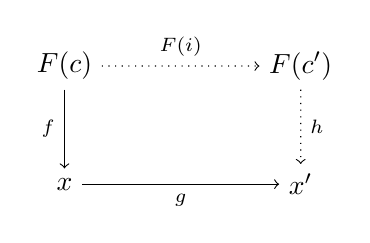
\begin{tikzpicture}[scale=1.5]
		\node (A) at (0,1) {$F(c)$};
		\node (B) at (2,1) {$F(c')$};
		\node (C) at (0,0) {$x$};
		\node (D) at (2,0) {$x'$};
		\path[->,font=\scriptsize,dotted]
		(A) edge node[above]{$F(i)$} (B)
		(B) edge node[right]{$h$} (D);
		\path[->,font=\scriptsize]
		(C) edge node[below]{$g$} (D)
		(A) edge node[left]{$f$} (C);
	\end{tikzpicture}
	\end{center}
	By induction hypothesis, $G,h\circ\sigma_{c'}^{-1},\Phi(c') \models P$. By naturality of $\sigma$ :
	\begin{center}
	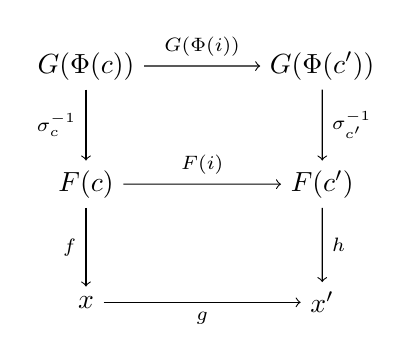
\begin{tikzpicture}[scale=1.5]
		\node (E) at (0,2) {$G(\Phi(c))$};
		\node (F) at (2,2) {$G(\Phi(c'))$};
		\node (A) at (0,1) {$F(c)$};
		\node (B) at (2,1) {$F(c')$};
		\node (C) at (0,0) {$x$};
		\node (D) at (2,0) {$x'$};
		\path[->,font=\scriptsize]
		(A) edge node[above]{$F(i)$} (B)
		(B) edge node[right]{$h$} (D)
		(C) edge node[below]{$g$} (D)
		(E) edge node[above]{$G(\Phi(i))$} (F)
		(E) edge node[left]{$\sigma_c^{-1}$} (A)
		(F) edge node[right]{$\sigma_{c'}^{-1}$} (B)
		(A) edge node[left]{$f$} (C);
	\end{tikzpicture}
	\end{center}
	So $G, f\circ\sigma_c^{-1},\Phi(c) \models \langle g \rangle P$.\\
	Conversely, if $G,f\circ\sigma_c^{-1},\Phi(c) \models \langle g \rangle P$ then there exists $\map{j}{\Phi(c)}{d'}$ in $\D$ and an isomorphism $\map{h}{G(d')}{x'}$ such that $h\circ G(j) = g\circ f\circ\sigma_c^{-1}$ and $G,h,d'\models P$.	
			\begin{center}
	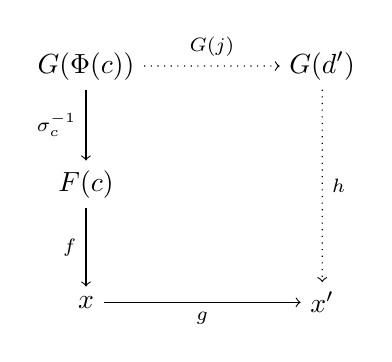
\begin{tikzpicture}[scale=1.5]
		\node (E) at (0,2) {$G(\Phi(c))$};
		\node (F) at (2,2) {$G(d')$};
		\node (A) at (0,1) {$F(c)$};
		%\node (B) at (2,1) {$F(c')$};
		\node (C) at (0,0) {$x$};
		\node (D) at (2,0) {$x'$};
		\path[->,font=\scriptsize,dotted]
		%(A) edge node[above]{$F(i)$} (B)
		(E) edge node[above]{$G(j)$} (F)
		(F) edge node[right]{$h$} (D);
		\path[->,font=\scriptsize]
		(E) edge node[left]{$\sigma_c^{-1}$} (A)
		(C) edge node[below]{$g$} (D)
		(A) edge node[left]{$f$} (C);
	\end{tikzpicture}
	\end{center}
	As $(\Phi,\sigma)$ is open, there exists $\map{i}{c}{c'}$ in $\C$ such that $\Phi(i) = j$ and $\Phi(c') = d'$. So $G,h,\Phi(c') \models P$ and by induction hypothesis, $F,h\circ\sigma_{c'},c' \models P$. Moreover, by naturality of $\sigma$ :
		\begin{center}
	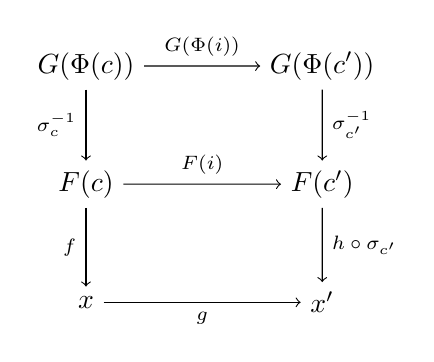
\begin{tikzpicture}[scale=1.5]
		\node (E) at (0,2) {$G(\Phi(c))$};
		\node (F) at (2,2) {$G(\Phi(c'))$};
		\node (A) at (0,1) {$F(c)$};
		\node (B) at (2,1) {$F(c')$};
		\node (C) at (0,0) {$x$};
		\node (D) at (2,0) {$x'$};
		\path[->,font=\scriptsize]
		(A) edge node[above]{$F(i)$} (B)
		(B) edge node[right]{$h\circ\sigma_{c'}$} (D)
		(C) edge node[below]{$g$} (D)
		(E) edge node[above]{$G(\Phi(i))$} (F)
		(E) edge node[left]{$\sigma_c^{-1}$} (A)
		(F) edge node[right]{$\sigma_{c'}^{-1}$} (B)
		(A) edge node[left]{$f$} (C);
	\end{tikzpicture}
	\end{center}
	So, $F,f,c \models \langle g \rangle P$.
			\item[$\star$] $F,f,c \models ?S$ iff $F,c \models S$ iff $G,\Phi(c) \models S$ iff $G,f\circ\sigma_c^{-1},\Phi(c) \models ?S$
			\item[$\star$] $F,f,c \models \neg P$ iff $F,f,c \not\models P$ iff $G,f\circ\sigma_c^{-1},\Phi(c)\not\models P$ iff $G,f\circ\sigma_c^{-1},\Phi(c)\models \neg P$
			\item[$\star$] $F,f,c \models \bigwedge\limits_{i\in I} P_i$ iff for all $i\in I$, $F,f,c \models P_i$ iff for all $i\in I$, $G,f\circ\sigma_c^{-1},\Phi(c) \models P_i$ iff $G,f\circ\sigma_c^{-1},\Phi(c) \models \bigwedge\limits_{i\in I} P_i$
		\end{itemize}
	From this and the surjectivity of $\Phi$, we deduce the result.
	
	
	
	\item[$\Leftarrow$] Conversely, suppose that $F$ and $G$ are logically equivalent. Define the relation:
	$$R = \{(c,f,d) \mid \forall S, (F,c \models S \Leftrightarrow G,d \models S), \map{f}{F(c)}{G(d)} ~ iso ~ s.t.$$
	$$~~~~~~~~~~~~~~~~~~~~f = h_2^{-1}\circ h_1 ~ with ~ h_1, h_2 ~ isos ~ and ~ \forall P, (F,h_1,c \models P \Leftrightarrow G,h_2,d \models P)\}$$
	We prove that $R$ is a bisimulation:
	\begin{itemize}
		\item[$\star$] Let $c$ be an object of $\C$. We exhibit an object $d$ of $\D$ and an isomorphism $\map{f}{F(c)}{G(d)}$ such that $(c,f,d) \in R$. Let $d$ such that for all object formulae $S$, $F,c \models S \Leftrightarrow G,d \models S$ (there exists at least one such a $d$ by the hypothesis). Let :
		$$Z = \{h \mid \map{h}{G(d)}{F(c)} ~ iso\}$$
		$Z$ is non empty : $F,c \models [F(c)]\top$ because $\map{id_{F(c)}}{F(c)}{F(c)}$ is an iso. So, $G,d \models [F(c)]\top$ and there exists an isomorphism $\map{h}{G(d)}{F(c)}$.
		
		Now, assume that there is no $h \in Z$ such that for all path formulae $F,id_{F(c)},c \models P$ iff $G,h,d \models P$. Then for all $h \in Z$, let $P_h$ be a formula such that $F,id_{F(c)},c \models P_h$ and $G,h,d \not\models P_h$ (we can always assume that we are in this case because we have negation). Then $F,c \models [F(c)]\bigwedge\limits_{h\in Z} P_h$ and $G,d \not\models [F(c)]\bigwedge\limits_{h\in Z} P_h$ which is absurd. So there is an isomorphism $\map{h}{G(d)}{F(c)}$ such that for all morphism formulae $P$, $F,id_{F(c)},c \models P$ iff $G,h,d \models P$. Then $(c,h^{-1},d) \in R$.
		\item[$\star$] Assume that we have :
		\begin{center}
	\begin{tikzpicture}[scale=1.5]
		\node (A') at (-1,0) {$c$};
		\node (A) at (0,0) {$F(c)$};
		\node (B) at (2,0) {$x$};
		\node (C) at (4,0) {$G(d)$};
		\node (C') at (5,0) {$d$};
		\node (D) at (0,2) {$F(c')$};
		\node (D') at (-1,2) {$c'$};
		\path[->,font=\scriptsize]
		(A) edge node[left]{$F(i)$} (D)
		(A') edge node[left]{$i$} (D')
		(A) edge node[below]{$h_1$} (B)
		(C) edge node[below]{$h_2$} (B);
	\end{tikzpicture}
	\end{center}
	with $h_1$, $h_2$ isos and for all morphism formulae $P$, $F,h_1,c \models P$ iff $G,h_2,d \models P$ (that is $(c,h_2^{-1}\circ h_1,d) \in R$). First, this diagram is commutative :
				\begin{center}
	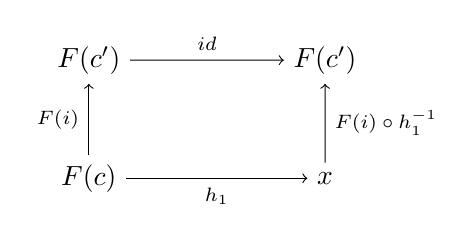
\begin{tikzpicture}[scale=1.5]
		\node (A) at (0,1) {$F(c')$};
		\node (B) at (2,1) {$F(c')$};
		\node (C) at (0,0) {$F(c)$};
		\node (D) at (2,0) {$x$};
		\path[->,font=\scriptsize]
		(A) edge node[above]{$id$} (B)
		(D) edge node[right]{$F(i)\circ h_1^{-1}$} (B);
		\path[->,font=\scriptsize]
		(C) edge node[below]{$h_1$} (D)
		(C) edge node[left]{$F(i)$} (A);
	\end{tikzpicture}
	\end{center}
	so $F,h_1,c \models \langle F(i)\circ h_1^{-1} \rangle \top$ and then $G,h_2,d \models \langle F(i)\circ h_1^{-1} \rangle \top$. So, the set :
	$$Z = \{(h,j) \mid \map{j}{d}{d'}, \map{h}{G(d')}{F(c')} ~ iso ~ such ~ that ~ F(i)\circ h_1^{-1}\circ h_2 = h \circ G(j)\}$$
	is non empty. Assume that there is no $(h,j) \in Z$ such that for all morphism formulae $P$, $F,id_{F(c')},c' \models P$ iff $G,h,d' \models P$. Then, for all $(h,j) \in Z$, let $P_{(h,j)}$ be a path formula such that $F,id_{F(c')},c' \models P_{(h,j)}$ and $G,h,d' \not\models P_{(h,j)}$. Then, $F,h_1,c \models \langle F(i)\circ h_1^{-1} \rangle \bigwedge\limits_{(h,j)\in Z} P_{(h,j)}$ and $G,h_2,d \not\models \langle F(i)\circ h_1^{-1} \rangle \bigwedge\limits_{(h,j)\in Z} P_{(h,j)}$ which is absurd. So there are $h$ and $j$ such that :
			\begin{center}
	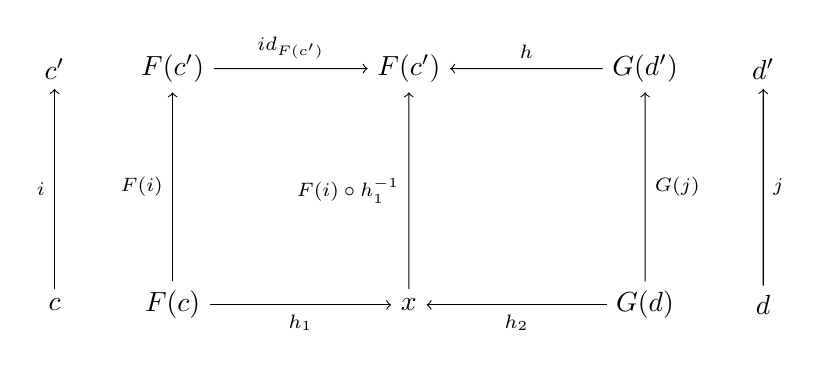
\begin{tikzpicture}[scale=1.5]
		\node (A') at (-1,0) {$c$};
		\node (A) at (0,0) {$F(c)$};
		\node (B) at (2,0) {$x$};
		\node (C) at (4,0) {$G(d)$};
		\node (C') at (5,0) {$d$};
		\node (D) at (0,2) {$F(c')$};
		\node (D') at (-1,2) {$c'$};
		\node (E) at (2,2) {$F(c')$};
		\node (F) at (4,2) {$G(d')$};
		\node (F') at (5,2) {$d'$};
		\path[->,font=\scriptsize]
		(C') edge node[right] {$j$} (F')
		(C) edge node[right] {$G(j)$} (F)
		(F) edge node[above]{$h$} (E)
		(D) edge node[above]{$id_{F(c')}$} (E)
		(B) edge node[left]{$F(i)\circ h_1^{-1}$} (E)
		(A) edge node[left]{$F(i)$} (D)
		(A') edge node[left]{$i$} (D')
		(A) edge node[below]{$h_1$} (B)
		(C) edge node[below]{$h_2$} (B);
	\end{tikzpicture}
	\end{center}
	and for all morphism formulae $P$, $F,id_{F(c')},c' \models P$ iff $G,h,d' \models P$. In particular, for all object formulae $S$, $F,id_{F(c')},c' \models ?S$ iff $G,h,d' \models ?S$ i.e. $F,c' \models S$ iff $G,d' \models S$ and so $(c',h^{-1},d') \in R$.
		\item[$\star$] the other two conditions are symmetric.
	\end{itemize}
\end{itemize}
\end{proof}






\section{Unfolding and po-diagrams}

In the previous chapter, we have seen that diagrams whose underlying category is a pre-order (the $\nathomolbw{n}{X}$ for example) were of particular interest. In this section, we prove that up to an operation of unfolding, everything can be made in those diagrams.

More precisely, by a \textbf{po-diagram} we will mean a diagram $\map{F}{\C}{\A}$ such that $\C$ is a preorder, i.e., a category whose Hom-sets are either empty, or a singleton. We denote by $\podiagr{\A}$ the full subcategory of $\diagriso{\A}$ consisting of po-diagrams.

We will first prove that a diagram is always bisimilar to a po-diagram, namely its \textbf{unfolding}. Given a diagram $\map{F}{\C}{\A}$, define its \textbf{unfolding} as the diagram $\map{\Unf{F}}{\Unf{\C}}{\A}$ such that:
\begin{itemize}
	\item[--] the objects of $\Unf{\C}$ are non-empty finite sequences $(f_1,...,f_n)$ of composable morphisms of $\C$, i.e., domain of $f_i$ = codomain of $f_{i-1}$,
	\item[--] the set of morphisms of $\Unf{\C}$ from $(f_1,...,f_n)$ to $(g_1,...,g_p)$ is $\{(g_{n+1},...,g_p)\}$ if $n \leq p$ and for all $i \leq n$, $f_i = g_i$, and is empty otherwise,
	\item[--] composition of $\Unf{\C}$ is concatenation,
	\item[--] identities of $\Unf{\C}$ are empty sequences,
	\item[--] $\Unf{F}(f_1,...,f_n) = F(c)$ where $c$ is the codomain of $f_n$,
	\item[--] $\Unf{F}(g_{n+1},...,g_p) = F(g_p\circ\ldots\circ g_{n+1})$.
\end{itemize}

From a more abstract viewpoint, the unfolding can be seen as follow: recall that $\PP$ is the subcategory of $\diagriso{\A}$ consisting of diagrams of the form $\map{B}{[n]}{\A}$. Consider the category $\PP\downarrow F$, i.e.:
\begin{itemize}
	\item whose objects are morphisms of the form $\map{(\Phi,id)}{(\map{B}{[n]}{\A})}{F}$ for some $\map{B}{[n]}{\A} \in \PP$,
	\item morphisms from $\map{(\Phi,\sigma)}{(\map{B}{[n]}{\A})}{F}$ to $\map{(\Phi',\sigma')}{(\map{B'}{[n']}{\A})}{F}$ are morphisms $\map{i_{n,m}}{(\map{B}{[n]}{\A})}{(\map{B'}{[n']}{\A})}$ such that $(\Phi',\sigma')\circ i_{n,m} = (\Phi,\sigma)$.
\end{itemize}
Formally, $\PP\downarrow F$ is not a comma category since we only consider morphisms $(\Phi,id)$, i.e., whose second component is a natural transformation consisting of identities. There is a functor $\map{\mathcal{U}}{\PP\downarrow F}{\diagriso{\A}}$ which maps $\map{(\Phi,\sigma)}{(\map{B}{[n]}{\A})}{F}$ to $\map{B}{[n]}{\A}$. Then $\Unf{F}$ is the colimit of $\mathcal{U}$. The idea is similar to Chapter 3. $\PP\downarrow F$ can be seen as the category of finite sequences $(f_1,...,f_n)$ of composable morphisms of $\C$ and the unfolding is just a glueing of all those data.

\begin{lemme}~
\label{unfold}
\begin{itemize}
	\item[i)] For all $F$, $\Unf{F}$ is well defined and is a po-diagram.
	\item[ii)] $\Unf{F}$ extends to a functor $\map{\Unfo}{\diagriso{\A}}{\podiagr{\A}}$.
	\item[iii)] $\Unfo$ preserves open maps, i.e., if $(\Phi,\sigma)$ is an open map then so is $\Unf{\Phi,\sigma}$.
\end{itemize}
\end{lemme}

\begin{proof}~
\begin{itemize}
	\item[i)] Easy.
	\item[ii)] Given a morphism of diagrams $(\Phi,\sigma)$ from $\map{F}{\C}{\A}$ to $\map{G}{\D}{\A}$, we define $\Unf{\Phi,\sigma} = (\Unf{\Phi},\Unf{\sigma})$ with:
		\begin{itemize}
			\item[--] $\Unf{\Phi}(f_1,...,f_n) = (\Phi(f_1),...,\Phi(f_n))$,
			\item[--] $\map{\Unf{\sigma}_{(f_1,...,f_n)} = \sigma_{\text{codom}(f_n)}}{F(codom(f_n))}{G\circ\Phi(codom(f_n))}$.
		\end{itemize}
		It is easy to check that $\Unf(\Phi)$ is a functor. Naturality of $\Unf(\sigma)$ comes from the naturality of $\sigma$.
	\item[iii)] Now assume that $(\Phi,\sigma)$ is open. 
		\begin{itemize}
			\item[--] \textbf{surjectivity on objects:} Let $(g_1,...,g_n)$ be a non-empty finite sequence of composable morphisms of $\D$. By surjectivity on objects of $\Phi$, there is an object $c_0$, of $\C$ such that $\Phi(c_0) = dom(g_1)$. Then by the lifting property of $\Phi$, there is a morphism $\map{f_1}{c_0}{c_1}$ of $\C$ such that $\Phi(f_1) = g_1$. We have $dom(g_2) = codom(g_1) = c_1$ so by the lifting property of $\Phi$ there is a morphism $f_2$ such that... By induction, we construct a non-empty finite sequence of composable morphisms of $\C$ such that for all $i$, $g_i = \Phi(f_i)$ and so $\Unf{\Phi}(f_1,...,f_n) = (g_1,...,g_n)$.
			\item[--] \textbf{lifting property:} the proof is the same as the previous point.
			\item[--] \textbf{$\Unf{\sigma}$ is a natural isomorphism:} because $\sigma$ is.
		\end{itemize}
\end{itemize}
\end{proof}

\begin{prop} If we denote the injection by $\map{\iota}{\podiagr{\A}}{\diagriso{\A}}$, there is a natural transformation $\map{\mu}{\iota\circ \Unfo}{id_{\diagriso{\A}}}$ such that for all $F$, $\mu_F$ is an open map.\\
In particular, $F$ and $\Unf(F)$ are bisimilar.
\end{prop}

One should remark that, nevertheless, $\Unfo$ is not a right adjoint of $\iota$.

\begin{proof}
Let $\map{F}{\C}{\A}$ be a diagram. We construct $\map{\mu_F = (\Phi_F,id)}{\Unf{F}}{F}$ as follow:
		\begin{itemize}
			\item[--] $\Phi_F(f_1,...,f_n) = codom(f_n)$
			\item[--] $\Phi_F(g_{n+1},...,g_p) = g_p \circ ... \circ g_{n+1}$
		\end{itemize}
		So, $\Unf(F) = F \circ \Phi_F$. Then:
		\begin{itemize}
			\item[--] \textbf{surjectivity on objects:} $\Phi_F(id_c) = c$,
			\item[--] \textbf{lifting property:} if we have a morphism $\map{f}{codom(f_n)}{c}$ then $(f)$ is a morphism from $(f_1,...,f_n)$ to $(f_1,...,f_n,f)$ such that $\Phi_F(f) = f$,
			\item[--] \textbf{$id$ is a natural isomorphism:} OK.
		\end{itemize}
		Naturality of $\mu$ is easy.
\end{proof}

\begin{coro}
Two diagrams $F$ and $G$ are bisimilar iff there are a po-diagram $H$ and a span of open maps $F \longleftarrow H \longrightarrow G$.
\end{coro}

\begin{proof}
If there is a span of open maps $F \xleftarrow{(\Phi,\sigma)} H \xrightarrow{(\Psi,\tau)} G$, then $F \xleftarrow{(\Phi,\sigma)\circ\mu_H} \Unf{H} \xrightarrow{(\Psi,\tau)\circ\mu_H} G$ is also a span of open maps since $\mu_H$ is open and open maps are closed under composition. Moreover $\Unf{H}$ is a po-diagram.
\end{proof}




\section{Grothendieck construction of a po-diagram}
	
	From now on, we will consider that $\A$ is a category of $\R$-modules for some ring $\R$.
	
	\subsection{Grothendieck construction of a po-diagram in modules}
	
	The Grothendieck construction (see for example \cite{johnstone02}) is a formal construction which maps any functor $\map{F}{\C}{\cat}$ from any small category $\C$ to the category of small categories to a category $\int F$, which is intuitively its category of elements. More precisely, $\int F$ is the category whose:
	\begin{itemize}
		\item objects are couples $(c,x)$ with $c$ an object of $\C$ and $x$ an object of $F(c)$,
		\item morphisms from $(c,x)$ to $(d,y)$ are couples $(f,g)$ with $\map{f}{c}{d}$ a morphism of $\C$ and $\map{g}{F(f)(x)}{y}$ morphism of $F(d)$,
		\item the identity of $(c,x)$ is $(id_c, id_x)$,
		\item composition is defined by $(f,g)\circ(f',g') = (f\circ f',g\circ F(f)(g'))$.
	\end{itemize}
	
%	When $F$ is with values in groups, i.e., small groupoids with one object, this definition can be simplified: since there is only one object, the second component in the objects of $\int F$ is useless. Moreover, is then $(f\circ f', g + F(f)(g'))$. When the underlying category $\C$ is a poset and $F$ is with values in abelian groups, the category $\int F$ can be equipped with a structure of partially enriched category in abelian groups. 

When $\map{F}{\C}{\A}$, $F$ can be seen as a functor $\map{F}{\C}{\cat}$: a module being an abelian group for the additive structure, it can be seen as a category with one object. So we can apply the Grothendieck construction on such a functor. When $\C$ is a poset the definition simplifies greatly as follow. $\int F$ is the category whose:
	\begin{itemize}
		\item objects are the objects of $\C$,
		\item morphisms from $c$ to $d$, with $c \leq d$, are the elements of $F(d)$,
		\item the identity of $c$ is $0_{F(c)}$,
		\item composition is defined by: for every $g' \in F(d)$ and $g \in F(e)$ with $c \leq d \leq e$, $g\circ g' = g + F(d\leq e)(g')$.
	\end{itemize}
By construction, Hom-sets have a structure of $\R$-modules. A stronger statement is the following:

\begin{prop}
When $\map{F}{\C}{\A}$ is a po-diagram, $\int F$ has the structure of a partially enriched category in $\A$.
\end{prop}

\begin{proof}
First, we must prove that the composition is bilinear: 
$$(\alpha.g_1+\beta.g_2)\circ (\alpha.g_1'+\beta.g_2') = \alpha.g_1 + \beta.g_2 + F(d\leq e)(\alpha.g_1'+\beta.g_2')$$ $$= \alpha.(g_1+F(d\leq e)(g_1')) + \beta.(g_2+F(d\leq e)(g_2')) = \alpha.(g_1\circ g_1') + \beta.(g_2\circ g_2')$$

Next, we must prove the axioms of a partially enriched category from section \ref{subsec:pec}:
		\begin{itemize}
			\item[--] (unit) can be expressed as: for all $ g \in F(d)$, $$g + F(c \leq d)(0) = g = F(d \leq d)(g) + 0$$ which is true because $F(d \leq d) = id$ since $F$ is a functor and $F(c \leq d)(0) = 0$ since $F(c \leq d)$ is a morphism of groups.
			\item[--] (associativity) can be expressed as for all $g \in F(d)$, $g' \in F(e)$ and $g'' \in F(f)$:
			$$F(e\leq f)(F(d\leq e)(g) + g') + g'' =$$
			$$F(e \leq f)(F(d\leq e)(g)) + F(e \leq f)(g') + g'' =$$
			$$F(d\leq f)(g) + F(e\leq f)(g') + g''$$
		\end{itemize}
\end{proof}

\begin{lemme}
$\int$ extends to a functor $\map{\int}{\podiagr{\A}}{\pecat{\A}}$.
\end{lemme}

\begin{proof}
If $(\Phi,\sigma)$ is a morphism of po-diagrams from $\map{F}{\C}{\A}$ to $\map{G}{\D}{\A}$, we define a partially enriched functor $\int(\Phi,\sigma)$ from $\int F$ to $\int G$ as follow:
	\begin{itemize}
		\item[--] the monotonous function part is $\Phi$,
		\item[--] for $c \leq c'$, $\map{\int(\Phi,\sigma)_{c,c'}}{F(c')}{G(\Phi(c'))}$ is $\sigma_{c'}$.
	\end{itemize}
	The first axiom of partially enriched functor comes from the naturality of $\sigma$ and the second is trivial.
\end{proof}

	
	
	
	\subsection{Extending equivalence of categories to partially enriched categories}
	
	We have seen in section \ref{subsec:pec} a notion of weak equivalences of partially enriched categories coming from the theory of model structures. Partially enriched categories being extensions of enriched categories and so of categories, there is another natural way to define that two partially enriched categories are equivalent by extending the notion of equivalence of categories. Usually, we say that two categories $\C$ and $\D$ are \textbf{equivalent} if there are two functors $\map{F}{\C}{\D}$ and $\map{G}{\D}{\C}$ and two natural isomorphisms $\map{\sigma}{F\circ G}{id_\D}$ and $\map{\tau}{G\circ F}{id_\C}$. This definition is equivalent (modulo the axiom of choice) to the fact that there is a functor $\map{F}{\C}{\D}$ which is:
	\begin{itemize}
		\item \textbf{fully faithful:} for every objects $c$, $c'$ of $\C$, the fonction $\map{F_{c,c'}}{\C(c,c')}{\D(F(c),F(c'))}$ is a bijection,
		\item \textbf{essentially surjective:} for every object $d$ of $\D$, there are an object $c$ of $\C$ and an isomorphism from $F(c)$ to $d$.
	\end{itemize}
	
	Equivalence of categories is extended to the enriched case by enriching either of the above equivalent characterization. In our case of partial enrichment, generalizing those definitions goes wrong for two reasons. First, because of partiality, natural transformations have no nice extensions. Secondly, already in the enriched case, this definition has a weird behavior in some cases. For example, when enriching in modules, essential surjectivity (or the existence of natural isomorphisms) becomes trivial, since neutral elements of the Hom-objects are always isomorphisms. For these reasons, we will not consider those characterizations but the following one:
	
	\begin{prop}
	Two categories $\C$ and $\D$ are equivalent iff there is a span $\C \xleftarrow{~ F ~} \E \xrightarrow{~ G ~} \D$ of functors which are:
	\begin{itemize}
		\item fully faithful,
		\item surjective on objects.
	\end{itemize}
	\end{prop}
	
	The main point is that we do not talk about isomorphisms of $\C$ and $\D$ anymore.
	
	\begin{proof}~
	\begin{itemize}
		\item[$\Leftarrow$] Obvious because surjectivity implies essential surjectivity.
		\item[$\Rightarrow$] Suppose that there is a fully faithful and essentially surjective functor $\map{F}{\C}{\D}$. Let $\E$ be the category whose:
		\begin{itemize}
			\item[$\star$] objects are tuples $(c,\theta,\eta,d)$ which satisfies the requirement of essential surjectivity, i.e., $\map{\theta}{F(c)}{d}$ is inverse of $\map{\eta}{d}{F(c)}$,
			\item[$\star$] the Hom-set $\E((c,\theta,\eta,d),(c',\theta',\eta',d'))$ is $\C(c,c')$,
			\item[$\star$] compositions and identities are those of $\C$.
		\end{itemize}
Let $\map{F_\C}{\E}{\C}$ be the functor such that:
		\begin{itemize}
			\item[$\star$] $F_C(c,\theta,\eta,d) = c$,
			\item[$\star$] $F_C((c,\theta,\eta,d),(c',\theta',\eta',d')) ~:~ {\E((c,\theta,\eta,d),(c',\theta',\eta',d'))}\longrightarrow {\C(c,c')}$ is $id_{\C(c,c')}$.
		\end{itemize}
It is fully faithful (obvious) and surjective because $(c,id_{F(c)},id_{F(c)},F(c))$ is an object of $\E$.

Let $\map{F_\D}{\E}{\D}$ be the functor such that:
		\begin{itemize}
			\item[$\star$] $F_\D(c,\theta,\eta,d) = d$,
			\item[$\star$] ${F_\D((c,\theta,\eta,d),(c',\theta',\eta',d'))} ~:~ {\E((c,\theta,\eta,d),(c',\theta',\eta',d'))}\longrightarrow {\D(d,d')}$ is the function $$f \longmapsto \theta'\circ F_{c,c'}(f)\circ \eta$$ which is a bijection with inverse $g \longmapsto F_{c,c'}^{-1}(\eta'\circ g\circ\theta)$.
		\end{itemize}
		It is fully faithful because $F$ is and surjective because $F$ is essentially surjective.
\end{itemize}
\end{proof}


\begin{defi}
We say that a partially enriched functor $\map{F}{\E}{\C}$ is:
\begin{itemize}
	\item[--] \textbf{fully-faithful} if for every pair $e \leq e'$ in $\E$, $\map{F_{e,e'}}{\E(e,e')}{\C(F(e),F(e'))}$ is an isomorphism,
	\item[--] \textbf{surjective} if $\map{F}{\ob{\E}}{\ob{\C}}$ is surjective,
	\item[--] \textbf{fibrational} if for every $e \in \ob{\E}$ and $c\in\ob{\C}$ such that $F(e) \leq c$ there is $e'$ such that $e \leq e'$ and $F(e') =c$.
\end{itemize}
We call \textbf{strong equivalence} any partially enriched functor which is fully-faithful, surjective and fibrational. We say that two partially enriched categories are \textbf{equivalent} if there is a span of strong equivalences between them.
\end{defi}

The last condition may seem a bit weird, but it is very important. Without the fibrational condition, this equivalence would be a bit trivial: taking a suitable $\E$ whose domain is equality would make equivalent two partially enriched categories which have the same endomorphisms. Moreover, the strong equivalences between two enriched categories (seen as partially enriched categories) are exactly the fully-faithful surjective enriched functors between them.

The following result was easy in the non-enriched case because of the several equivalent formulations, but now it must be proved:

\begin{prop}
Equivalence of partially enriched categories is an equivalence relation.
\end{prop}

\begin{proof}
Reflexivity and symmetry are obvious. The only interesting part is transitivity, i.e., assume that we have four strong equivalences as follow:
		\begin{center}
	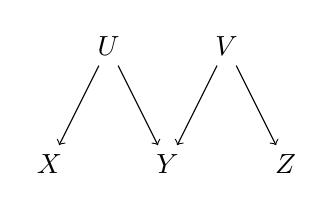
\begin{tikzpicture}[scale=1.5]
		\node (X) at (0,0) {$X$};
		\node (Y) at (1,0) {$Y$};
		\node (Z) at (2,0) {$Z$};
		\node (U) at (0.5,1) {$U$};
		\node (V) at (1.5,1) {$V$};
		\path[->,font=\scriptsize]
		(U) edge (X)
		(U) edge (Y)
		(V) edge (Y)
		(V) edge (Z);
	\end{tikzpicture}
	\end{center}
then we must construct two strong equivalences as follow:
		\begin{center}
	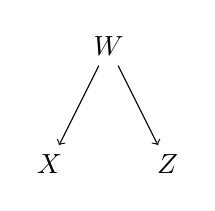
\begin{tikzpicture}[scale=1.5]
		\node (X) at (0,0) {$X$};
		\node (Z) at (1,0) {$Z$};
		\node (W) at (0.5,1) {$W$};
		\path[->,font=\scriptsize]
		(W) edge (X)
		(W) edge (Z);
	\end{tikzpicture}
	\end{center}
As strong equivalences are closed by composition, it is enough to prove the following. Assume that we have two strong equivalences as follow:
		\begin{center}
	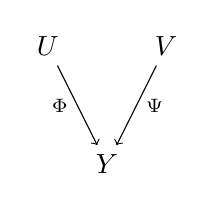
\begin{tikzpicture}[scale=1.5]
		\node (Y) at (0,0) {$Y$};
		\node (U) at (-0.5,1) {$U$};
		\node (V) at (0.5,1) {$V$};
		\path[->,font=\scriptsize]
		(U) edge node[left]{$\Phi$} (Y)
		(V) edge node[right]{$\Psi$} (Y);
	\end{tikzpicture}
	\end{center}
then we must construct two other strong equivalences as follow:
		\begin{center}
	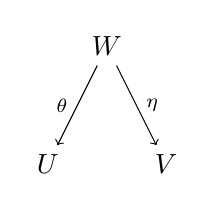
\begin{tikzpicture}[scale=1.5]
		\node (X) at (0,0) {$U$};
		\node (Z) at (1,0) {$V$};
		\node (W) at (0.5,1) {$W$};
		\path[->,font=\scriptsize]
		(W) edge node[left]{$\theta$} (X)
		(W) edge node[right]{$\eta$} (Z);
	\end{tikzpicture}
	\end{center}
Construct the partially enriched category $W$ whose:
\begin{itemize}
	\item objects are pairs of $(u,v)$ with $u$ object of $U$ and $v$ object of $V$ such that $\Phi(u) = \Psi(v)$,
	\item its domain is $(u,v) \leq (u',v')$ iff $u \leq u'$ and $v \leq v'$,
	\item Hom-object $W((u,v),(u',v')) = Y(\Phi(u),\Phi(u')) = Y(\Psi(v),\Psi(v'))$ (well defined for $u \leq u'$ and $v \leq v'$);
	\item compositions and identities are those of $Y$.
\end{itemize}
Define the partially enriched functor $\map{\theta}{W}{U}$ such that:
\begin{itemize}
	\item $\theta(u,v) = u$,
	\item $\map{\theta_{(u,v),(u',v')}}{Y(\Phi(u),\Phi(u'))}{U(u,u')} = \Phi_{u,u'}^{-1}$.
\end{itemize}
It is a strong equivalence:
\begin{itemize}
	\item \textbf{fully-faithful} obvious,
	\item \textbf{surjective} $\theta$ is surjective because $\Psi$ is,
	\item \textbf{fibrational} given $u \leq u'$ and $v$ such that $\Phi(u) = \Psi(v)$, then $\Psi(v) = \Phi(u) \leq \Phi(u')$ and as $\Psi$ is fibrational, there is $v'$ such that $v \leq v'$ and $\Psi(v') = \Phi(u')$ that is $(u',v')$ is an object of $W$, $\theta(u',v') = u'$ and $(u,v) \leq (u',v')$.
\end{itemize}
We construct a strong equivalence $\map{\eta}{W}{V}$ the same way.
\end{proof}

	\subsection{Relating bisimulation and equivalence of Grothendieck construction}
	
	First, we prove that the Grothendieck construction sends open morphism to equivalences:
	
	\begin{prop}
	If $(\Phi,\sigma)$ is an open morphism between po-diagrams, then $\int (\Phi,\sigma)$ is a strong equivalence. Consequently, if two po-diagrams are bisimilar, then their Grothendieck constructions are equivalent.
	\end{prop}
	
	\begin{proof}
	Assume that $(\Phi,\sigma)$ is open between po-diagrams. Let us prove that $\int(\Phi,\sigma)$ is a strong equivalence:
		\begin{itemize}
			\item[--] \textbf{surjectivity:} comes from the surjectivity on $\Phi$.
			\item[--] \textbf{fibrationality:} comes from the lifting property of $\Phi$.
			\item[--] \textbf{fully-faithful:} comes from the fact that $\sigma$ is a natural isomorphism.
		\end{itemize}
	If two po-diagrams are bisimilar, then there is span of open morphisms whose tip is also a po-diagram. Then we deduce the result by applying the functor $\int$.
	\end{proof}
	
	Reciprocally, we would like to prove that if the Grothendieck constructions of two po-diagram are equivalent, then they are bisimilar. It is done as follow: assume that $\map{F}{\C}{\A}$ and $\map{G}{\D}{\A}$ are two po-diagrams and that there is a span of strong equivalences $\int F \xleftarrow{~ K ~ } \M \xrightarrow{~ L ~} \int G$, where $\M$ is partially enriched category on $\A$. Let us start by constructing a diagram $\map{H}{\E}{\A}$ from $\M$ as follow:
	\begin{itemize}
		\item $\E$ is the set $\{(e,e')\mid e, e' \in \ob{\M} \wedge e \leq e'\}$ equipped with the preorder $(e,e') \sqsubseteq (e'',e''')$ iff $e = e''$ and $e' \leq e'''$,
		\item $H(e,e') = \M(e,e')$,
		\item $\map{H((e,e') \sqsubseteq (e,e''))}{\M(e,e')}{\M(e,e'')}$ is the morphism of groups that maps $g \in \M(e,e')$ to $\circ_{e,e',e''}(g,0_{\M(e',e'')})$.
	\end{itemize}

Let us prove that this is a functor:
\begin{itemize}
	\item $H((e,e') \leq (e,e'))(g) = \circ_{e,e',e'}(g,0_{\M(e',e')}) $\\$=\circ_{e,e',e'}(g,u_{e'}(0)) = g$ by (unit).
	\item $H((e,e'') \leq (e,e''')) \circ H((e,e') \leq (e,e''))(g) $\\$=H((e,e'') \leq (e,e'''))(\circ_{e,e',e''}(g,0_{\M(e',e'')}))$\\$=\circ_{e',e'',e'''}(\circ_{e,e',e''}(g,0_{\M(e',e'')}),0_{\M(e'',e''')}) $\\$=\circ_{e,e',e'''}(g,\circ_{e',e'',e'''}(0_{\M(e',e'')},0_{\M(e'',e''')}))$ by (associativity)\\
	$= \circ_{e,e',e'''}(g,0_{\M(e',e''')})$ because $\circ_{e',e'',e'''}$ is a morphism of groups\\
	$= H((e,e') \leq (e,e'''))(g)$.
\end{itemize}

Let us define an open map $(\Phi,\sigma)$ from $H$ to $F$ as follow:
	\begin{itemize}
		\item $\Phi(e,e') = K(e')$ (which is monotonous),
		\item for every $e \leq e'$, $\map{\sigma_{(e,e')}}{\M(e,e')}{F(K(e'))= \int F(K(e),K(e'))}$ is $K_{e,e'}$ 
	\end{itemize}
	Let us prove that this is a well defined open map:
		\begin{itemize}
			\item \textbf{naturality of $\sigma$:} it can be reformulated as for every $e \leq e' \leq e''$, for every $g \in \M(e,e')$, \\$K_{e,e'}(H((e,e') \leq (e,e'')) (g)) = K_{e,e''}(\circ_{e,e',e''}(g,0))$\\$= \circ_{K(e),K(e'),K(e'')}(K_{e,e'}(g),K_{e,e''}(0))$ because $K$ is a partially enriched functor\\
			$= \circ_{K(e),K(e'),K(e'')}(K_{e,e'}(g),0)$ because $K_{e,e''}$ is a morphism of groups\\
			$=F(e' \leq e'')(K_{e,e'}(g))$ by definition of the composition in $\int F$.
			\item \textbf{surjectivity:} comes from the surjectivity of $K$.
			\item \textbf{lifting property:} comes from the fibrational condition of $K$.
			\item \textbf{$\sigma$ natural isomorphism:} comes from the fully-faithfulness of $K$.
		\end{itemize}
The same way, one can construct an open map from $H$ to $G$. Consequently:

\begin{theo}
Two po-diagrams are bisimilar iff their Grothendieck constructions are equivalent.
Two diagrams are bisimilar iff the Grothendieck construction of their unfoldings are equivalent.
\end{theo}





\section{Decidability}
\label{sec:deci}

The end of this chapter is dedicated to proving some decidability results on bisimilarity and diagramatic logic in the case of modules, more particularly, in real and rational vector spaces. The main idea of those results will be to reduce our problems to the existence of some invertible matrices satisfying linear conditions. In the present section, we focus on an existential theory of matrices. We first recall the case of the existential theory of the reals, known to be decidable. We then introduce the existential theory of invertible matrices in $\mathbb{R}$ and $\mathbb{Q}$ and we prove the decidability of their satisfiability problems.

\subsection{The existential theory of some rings}

Designing algorithms for finding solutions of equations is a old problem in mathematics. The famous Hilbert's tenth problem posed the problem for polynomial equations in integers, but the question can be asked for other rings. Tarski in \cite{tarski51} solved this question for the reals: the first-order logic of real closed fields is decidable, although the solution being of non-elementary complexity. Improvement had be done: it was proved to be in EXPSPACE in \cite{benor86} and that the existential theory of the reals is in PSPACE in \cite{canny88}. On the other hand, Matiyasevich's negative answer of the tenth problem, means that the existential theory of the integers is undecidable. In particular, since it is possible to express that a rational is an integer (using possibly universal quantifiers), the full first-order logic of the rationals is undecidable. However, it is still an open question whether its existential fragment is decidable or not.

\subsection{Theory of matrices}

In this section, we will consider a logic of matrices that will be expressible in the existential theory of the reals. It will be the main ingredient to decide some problems in diagrams with values in vector spaces. Namely, we consider formulae of the form:
$$\exists_{n_1}X_1.\ldots.\exists_{n_k}X_k. \bigwedge\limits_{j = 1}^m P_j(X_1, \ldots, X_k)$$
where:
\begin{itemize}
	\item $n_i \geq 0$, is an integer,
	\item $P_j$ is a predicate of the form $A.X_i = X_j.B$ for some $i$, $j$ and matrices $A$, $B$ with coefficients in rationals, $A$ of size $n_j\times n_i$, and $B$ of size $n_i\times n_j$.
\end{itemize}
We call it the \textbf{existential theory of invertible matrices}.

We will consider the following decision problem: given such a formula, is it satisfiable, that is, are there matrices $M_1$, ..., $M_k$, with $M_i$ of size $n_i\times n_i$, invertible such that for every $j$, $P_j(M_1, ..., M_k)$ is true ?

We may ask this question for matrices $M_i$ in the reals or the rationals. We will prove that the two problems actually coincide and are decidable in PSPACE.


\subsection{Decidability in $\mathbb{R}$}

We stick here to the case of the reals. We prove that we have a reduction to the existential theory of the reals. Given a formula
$$\Phi = \exists_{n_1}X_1.\ldots.\exists_{n_k}X_k. \bigwedge\limits_{j = 1}^m P_j(X_1, \ldots, X_k)$$
we will construct a formula $\Psi$ in the existential theory of the reals which is satisfiable if and only if $\Phi$ is.

First, for every quantifier $\exists_{n_i}X_i$, we fix $2.n_i^2$ fresh first-order variables $x_i^{r,s}$ and $y_i^{r,s}$ for $r,s \in \{1, ..., n_i\}$. Let $X_i$ be the matrix of size $n_i\times n_i$ whose coefficients are $x_i^{r,s}$, and $Y_i$ whose coefficients are $y_i^{r,s}$. Developing $A.X_i = X_j.B$ leads to $n_jn_i$ linear equations on the variables $x_i^{r,s}$ and $x_j^{r,s}$. So every predicate $P_j$ induces a set $L_j$ of linear equations. It remains to express that $X_i$ is invertible in first-order logic. The idea is to express that $Y_i$ is its inverse. Developing $X_i.Y_i = \text{Id}$ and $Y_i.X_i = \text{Id}$, leads to $2.n_i^2$ polynomial equations on the variables $x_i^{r,s}$ and $y_i^{r,s}$. Let $S_i$ be this set. We note $\Psi$ the formula:
$$\exists x_1^{1,1}.\ldots\exists x_k^{n_k,n_k}. \bigwedge\limits_{i=1}^k S_i \wedge \bigwedge\limits_{j=1}^m L_j$$
$\Psi$ is of polynomial size on the size of $\Phi$.

\begin{prop}
$\Psi$ is satisfiable in the existential theory of the reals iff $\Phi$ is satisfiable in the existential theory of invertible matrices in the reals. Consequently, the existential theory of invertible matrices in the reals is decidable in PSPACE.
\end{prop}

\subsection{The rational case}

As we have seen previously, first-order theories of rationals are harder in general. But there are some algebraic problems that are known to coincide when considering the reals and the rationals.

Given a linear system with coefficients in rationals, gaussian elimination works independently of the coefficient field. Consequently, the real subspace $F_{\mathbb{R}}$ of solutions of this system has the same dimension as the rational subspace $F_{\mathbb{Q}}$ of solutions of the system. Actually, $F_{\mathbb{R}}\cap \mathbb{Q}^n = F_{\mathbb{Q}}$ and they have a common basis whose vectors are in the rationals.

Similarly, the problem of equivalence of matrices coincides in the reals and the rationals. Given two matrices $A$ and $B$ with coefficients in the rationals, $A$ and $B$ are equivalent if there are two invertible matrices $X$ and $Y$ such that $A.X = Y.B$. This problem is also solvable using gaussian elimination by computing the rank of $A$ and $B$, which is independent of the coefficient field.

Our problem is a generalization of the equivalence problem and the same kind of results hold here:

\begin{prop}
A formula $\Phi$ is satisfiable in the existential theory of invertible matrices in the reals if and only if it is satisfiable in the rationals.
\end{prop}

\begin{proof}
Let $\Phi$ be a formula which is satisfiable in the reals. It is enough to prove that the formula $\Psi$ constructed in the previous subsection has a model in the rationals. We have seen that the satisfiability problem reduces to solving a linear system $\bigwedge\limits_{j=1}^m L_j$ in $\mathbb{R}^{n_1^2+\ldots+n_k^2}$, with the constraints that some matrices are invertible. Since $\Psi$ is satisfiable, the linear system $\bigwedge\limits_{j=1}^m L_j$ has a non trivial subspace $F$ of solution in the reals. Let $p$ be its dimension and $t_1$, ..., $t_p$ a basis (which is in the rationals, since the system is with coefficients in the rationals). 
There is then an isomorphism $\map{\kappa}{F}{\mathbb{R}^p}$. The set of solution of $\bigwedge\limits_{i=1}^k S_i \wedge \bigwedge\limits_{j=1}^m L_j$ in the reals is a subset $S$ of $F$. It is enough to prove that $S$ is a non-empty open set of $F$ (with any topology coming from a norm). Indeed, in this case, the image $\kappa(S)$ is then a non-empty open set of $\mathbb{R}^p$. Since, $\mathbb{Q}^p$ is dense in $\mathbb{R}^p$, $\kappa(S)$ intersects $\mathbb{Q}^p$ and there is $(s_1,\ldots,s_p) \in \kappa(S)\cap\mathbb{Q}^p$. Then, $s_1.t_1 + \ldots + s_p.t_p$ is a vector of rationals which is solution of $\bigwedge\limits_{i=1}^k S_i \wedge \bigwedge\limits_{j=1}^m L_j$.

It remains to prove that $S$ is open in $F$. So it is enough to prove that the set of solutions $T_i$ of $S_i$ is an open set of $\mathbb{R}^{n_1^2+\ldots+n_k^2}$. $T_i$ is of the form $\mathbb{R}^{n_1^2+\ldots+n_{i-1}^2}\times \text{Inv}_{n_i} \times \mathbb{R}^{n_{i+1}^2+\ldots+n_p^2}$, where $\text{Inv}_{n_i}$ is the set of invertible matrices in the reals of size $n_i\times n_i$.  $Inv_{n_i}$ is the inverse image of $\mathbb{R}\setminus\{0\}$ by the determinant function, which is continuous. Consequently, $\text{Inv}_{n_i}$ is open, and $T_i$ is open.
\end{proof}

\subsection{Further discussions on integers}

A natural question would be: what about integers ? We know that their existential theory is undecidable, so the line of proof in the case of the reals cannot apply here. The result on the rationals tends to imply that we do not use the full power of the existential fragment. Nevertheless, contrary to the rationals, the theory of matrices in integers is more complicated. For example, the equivalence of matrices is not solved by the rank, but by invariant factors, computed by an extension of the gaussian elimination, the Smith normal form. So it is an open question whether the existential theory of invertible matrices in integers is decidable or not.



\subsection{Finitary diagrams and formulae}

Finally, we prove a few decidability results for bisimilarity of diagrams and diagramatic logic using the existential theory of invertible matrices. In this section, we consider diagrams with values in real vector spaces (or rational, but as we have seen in the previous section, the two theories will coincide). We first describe the diagrams and the formulae used, the finitary diagrams and formulae. We then prove the decidability of two following problems:
\begin{itemize}
	\item \textbf{bisimilarity:} given two finitary diagrams, are they bisimilar ?
	\item \textbf{diagram model-checking:} given a finitary diagram $F$, an object $c$ of its domain and a positive finitary state formula $S$, $F,c \vDash S$ ? 
\end{itemize}



In our work on directed algebraic topology, the finite diagrams produced in \cite{dubut15} are of a particular form: their domain is a poset and they are with values in finite dimensional real (or rational) vector spaces. Consequently, we are particularly interested in deciding whether two such diagrams are bisimilar. We then call \textbf{finitary diagram} $F$ the following data:
\begin{itemize}
	\item a finite poset $\C$, $\leq$, which will be called the \textbf{domain},
	\item for every element $c$ of $\C$, an integer $F(c)$ (which stands for the real vector space $\mathbb{R}^{F(c)}$),
	\item for every pair $c \leq c'$ of $\C$, a matrix $F(c\leq c')$ of size $F(c)\times F(c')$, with coefficient in the rationals,
\end{itemize}
such that:
\begin{itemize}
	\item $F(c\leq c)$ is the identity matrix,
	\item for every triple $c \leq c' \leq c''$, $F(c\leq c'') = F(c'\leq c'').F(c\leq c')$.
\end{itemize}

Similarly, we are interested in model-checking of such diagrams because it may be simpler to just provide a formula from diagramatic logic as a witness that two diagrams are not bisimilar. We will consider the formulae generated by the following grammar, called \textbf{finitary formulae}:
$$\text{\textbf{Object formulae:~~}} S::=[n]P~~~~~n\in\mathbb{N}$$
$$\text{\textbf{Morphism formulae:~~}} P::=\langle M \rangle P\mid?S\mid\neg P\mid \top \mid P_1\wedge P_2~~~~M \text{ matrix in the rationals}$$
Here, $[n]P$ stands for $[\mathbb{R}^n]P$ which makes finitary formulae diagramatic formulae in real vector spaces. This time, since we only have finitely branching diagrams, we only consider finite conjunctions. We will more particularly consider \textbf{positive} formulae, i.e., formulae that do not use negation.

For both problem, the main idea will be to construct non-deterministically a formula of the existential theory of invertible matrices and to check it using the previous section.



\subsection{Decidability of bisimilarity}

We start with the bisimilarity problem. Given two finitary diagrams $F$ and $G$, with domain $\C$, $\leq$ and $\D$, $\preceq$ respectively. The idea is to construct non-deterministically a bisimulation $R$, that is, a set of triples $(c,M,d)$ where $M$ is a matrix in the reals (or the rationals) satisfying the properties of a bisimulation from Section 2, except that we will not construct explicitly the matrices $M$, but a formula in the existential theory of invertible matrices that encodes that there exist some matrices $M$ such that the bisimulation constructed satisfies those properties.

\begin{algorithm}[h!]
\caption{Bisimilarity of finitary diagrams}
\begin{algorithmic}[1]
\Require Two finitary diagrams $\map{F}{\C}{\A}$ and $\map{G}{\D}{\A}$.
\Ensure Answer \textbf{Yes} iff $F$ and $G$ are bisimilar.
\State $S := \C\sqcup\D$;
\State $R := \varnothing$;
\State $lin := \varnothing$;
\State $var := \varnothing$;
\While{$S$ is non empty} 
	\State Pick some $c \in S$. Let us assume that $c \in \C$, the other case is symmetric.
	\State Non-deterministically choose $d \in \D$ with $F(c) = G(d) = n$. 
	\If{$d$ does not exist}
		\State\textbf{FAIL}
	\EndIf
	\State $S := S\setminus\{c,d\}$;
	\State Create a fresh variable $X$ and add the pair $(X,n)$ to $var$;
	\State Add $(c,X,d)$ to $R$ and do not mark it;
	\While{there is a non-marked element in $R$}
		\State Pick a non-marked element $(c,X,d) \in R$, with $F(c) = G(d) = n$;
		\State Mark $(c,X,d)$;
		\ForAll{$c' > c$}
			\State Non-deterministically choose $d \succeq d'$ with $F(c') = G(d') = m$.
			\If{$d'$ does not exist}
				\State\textbf{FAIL}
			\EndIf
			\State $S := S\setminus\{c',d'\}$;
			\State Create a fresh variable $X'$ and add the pair $(X',m)$;
			\State Add $(c',X',d')$ to $R$ and do not mark it;
			\State Add the equation $G(d\leq d').X = X'.F(c\leq c')$ to $lin$;
		\EndFor
		\ForAll{$d \prec d'$}
		\State Symmetrically
		\EndFor
	\EndWhile
\EndWhile
\State Let $\Phi$ be the formula of the existential theory of invertible matrices existentially quantified by $\exists_n X$ for every $(X,n) \in var$ and whose predicate are the linear equations from $lin$.
\State\Return \textbf{Yes} if $\Phi$ is valid, \textbf{No} otherwise.
\end{algorithmic}
\label{alg:algo1}
\end{algorithm}

Consider the algorithm \ref{alg:algo1} written in pseudo-code. It maintains the bisimulation $R$ and two sets $var$, encoding the variables of the formula we are constructing and $lin$, encoding its predicates.

The algorithm always terminates. First, the inner while loop terminates since after every loop an element $(c,X,d)$ is marked and only elements of the form $(c',X',d')$ with either $c < c'$ and $d \preceq d'$ or $c \leq c'$ and $d \prec d'$ are added. The outer loop terminates since after every loop at least one element of $S$ is removed.

Assume that there is an execution of the algorithm that answers \textbf{Yes}. Let $R$ and $\Phi$ constructed during this execution. Since the algorithm answers \textbf{Yes}, the formula $\Phi$ is satisfiable, that is, for every $(X,n) \in var$, there is an invertible matrix $M_X$ of size $n\times n$ such that for every equation $A.X=X'.B$ in $lin$, $A.M_X = M_{X'}.B$ holds. Let $R'$ be the set 
$$\{(c,M_X,d) \mid (c,X,d) \in R\}$$
Then by construction of $R$ and $\Phi$, $R'$ is a bisimulation between $F$ and $G$.

 Assume that there is a bisimulation $R'$ between $F$ and $G$. We show that there are non-deterministic choices that lead to the answer \textbf{Yes}. The idea is to assure that every $(c,X,d)$ that belongs to $R$ at some point corresponds to an element $(c,f,d)$ of $R'$. To assure this, we must:
\begin{enumerate}
	\item when choosing $d$ in line $7$, choose it such that there is $(c,f,d) \in R'$. It exists by definition of a bisimulation.
	\item when choosing $d'$ in line $18$, choose it in such a way that there is $(c',f',d')$ in $R'$ and that the element $(c,f,d) \in R'$ corresponding to $(c,X,d)$ satisfies that $G(d\leq d')\circ f = f'\circ F(c\leq c')$. Such a $d'$ always exist since $R'$ is a bisimulation.
\end{enumerate}
With this, the algorithm does not \textbf{FAIL} and the formula $\Phi$ is valid: the assignment that maps $X$ to the corresponding $f$ satisfies $\Phi$. Consequently, the algorithm answers \textbf{Yes}.

Finally, this algorithm non-deterministically constructs in exponential space a formula of exponential size in the size of the data. By Theorem 5, this algorithm is in NEXPSPACE. Consequently, since NEXPSPACE = EXPSPACE:
\begin{theo}
Knowing if two finitary diagrams are bisimilar in the reals or in the rationals is decidable in EXPSPACE. Furthermore, they are bisimilar in the reals if and only if they are bisimilar in the rationals.
\end{theo}


\subsection{Decidability of the model checking}

\subsubsection{Positive case}

We start with the positive fragment. So starting with a finitary diagram $F$, an element $c$ of its domain, and a positive finitary object formula $S$, we inductively construct two lists, initially empty:
\begin{itemize}
	\item $var$ of pairs $(X,n)$ where $X$ is a variable and $n$ an integer. This will stand for $\exists_n X$,
	\item $lin$ of equations $A.X=Y.B$ where $X$ and $Y$ are variables and $A$ and $B$ are matrices,
\end{itemize}
as previously.

The formula $S$ is of the form $[n]P$. We first check if $n = F(c)$. If it is not the case then we fail. Otherwise, let $X$ be a fresh variable. Add the pair $(X,n)$ to $var$. Continue with $F$, $c$, $X$ and $P$.

Now, assume that we consider the following data: a finitary diagram $F$, an element of its domain $c$, a variable $X$ in $var$ and a positive finitary morphism formula $P$. Several case:
\begin{itemize}
	\item if $P = ?S'$, continue with $F$, $c$ and $S'$,
	\item if $P = \top$, stop,
	\item if $P = P_1\wedge P_2$, first continue with $F$, $c$, $X$ and $P_1$. When this part terminates, continue with $F$, $c$, $X$ and $P_2$,
	\item if $P = \langle M \rangle P'$, with $M$ of size $n_1\times n_2$. If $n_1 \neq F(c)$, then we fail. Otherwise, non-deterministically choose an element $c' \geq c$, with $F(c') = n_2$. If such a $c'$ does not exist, then we fail. Finally, create a fresh variable $X'$, add $(X',n_2)$ to $var$ and $M.X = X'.F(c\leq c')$ to $lin$.
\end{itemize}

If the algorithm does not fail, construct a formula $\Phi$ from $var$ and $lin$ as previously and check if it is satisfiable using the existential theory of invertible matrices. The formula $\Phi$ is non-deterministically constructed in polynomial time and so is of polynomial size. So, this algorithm is in NPSPACE and since NPSPACE = PSPACE:
\begin{theo}
Knowing if a finitary diagram satisfies a positive finitary formula (either in the reals or in the rationals) is decidable in PSPACE.
\end{theo}

\subsubsection{Full case}

The full case is also decidable for the reals. The idea is similar, except that, because of the negation, it is not possible to encode our problem in the existential fragment. However, using the same ideas, it is still possible to encode it in the full first-order theory of real closed fields. There are two counter-parts:
\begin{itemize}
	\item first, since the full first-order theory is decidable in EXPSPACE, the full model-checking in the reals is in EXPSPACE,
	\item secondly, theorem 6 does not hold anymore and nothing can be said about the rational case.
\end{itemize}








